% Options for packages loaded elsewhere
\PassOptionsToPackage{unicode}{hyperref}
\PassOptionsToPackage{hyphens}{url}
\PassOptionsToPackage{dvipsnames,svgnames,x11names}{xcolor}
%
\documentclass[
]{article}

\usepackage{amsmath,amssymb}
\usepackage{iftex}
\ifPDFTeX
  \usepackage[T1]{fontenc}
  \usepackage[utf8]{inputenc}
  \usepackage{textcomp} % provide euro and other symbols
\else % if luatex or xetex
  \usepackage{unicode-math}
  \defaultfontfeatures{Scale=MatchLowercase}
  \defaultfontfeatures[\rmfamily]{Ligatures=TeX,Scale=1}
\fi
\usepackage{lmodern}
\ifPDFTeX\else  
    % xetex/luatex font selection
\fi
% Use upquote if available, for straight quotes in verbatim environments
\IfFileExists{upquote.sty}{\usepackage{upquote}}{}
\IfFileExists{microtype.sty}{% use microtype if available
  \usepackage[]{microtype}
  \UseMicrotypeSet[protrusion]{basicmath} % disable protrusion for tt fonts
}{}
\makeatletter
\@ifundefined{KOMAClassName}{% if non-KOMA class
  \IfFileExists{parskip.sty}{%
    \usepackage{parskip}
  }{% else
    \setlength{\parindent}{0pt}
    \setlength{\parskip}{6pt plus 2pt minus 1pt}}
}{% if KOMA class
  \KOMAoptions{parskip=half}}
\makeatother
\usepackage{xcolor}
\setlength{\emergencystretch}{3em} % prevent overfull lines
\setcounter{secnumdepth}{5}
% Make \paragraph and \subparagraph free-standing
\makeatletter
\ifx\paragraph\undefined\else
  \let\oldparagraph\paragraph
  \renewcommand{\paragraph}{
    \@ifstar
      \xxxParagraphStar
      \xxxParagraphNoStar
  }
  \newcommand{\xxxParagraphStar}[1]{\oldparagraph*{#1}\mbox{}}
  \newcommand{\xxxParagraphNoStar}[1]{\oldparagraph{#1}\mbox{}}
\fi
\ifx\subparagraph\undefined\else
  \let\oldsubparagraph\subparagraph
  \renewcommand{\subparagraph}{
    \@ifstar
      \xxxSubParagraphStar
      \xxxSubParagraphNoStar
  }
  \newcommand{\xxxSubParagraphStar}[1]{\oldsubparagraph*{#1}\mbox{}}
  \newcommand{\xxxSubParagraphNoStar}[1]{\oldsubparagraph{#1}\mbox{}}
\fi
\makeatother


\providecommand{\tightlist}{%
  \setlength{\itemsep}{0pt}\setlength{\parskip}{0pt}}\usepackage{longtable,booktabs,array}
\usepackage{calc} % for calculating minipage widths
% Correct order of tables after \paragraph or \subparagraph
\usepackage{etoolbox}
\makeatletter
\patchcmd\longtable{\par}{\if@noskipsec\mbox{}\fi\par}{}{}
\makeatother
% Allow footnotes in longtable head/foot
\IfFileExists{footnotehyper.sty}{\usepackage{footnotehyper}}{\usepackage{footnote}}
\makesavenoteenv{longtable}
\usepackage{graphicx}
\makeatletter
\newsavebox\pandoc@box
\newcommand*\pandocbounded[1]{% scales image to fit in text height/width
  \sbox\pandoc@box{#1}%
  \Gscale@div\@tempa{\textheight}{\dimexpr\ht\pandoc@box+\dp\pandoc@box\relax}%
  \Gscale@div\@tempb{\linewidth}{\wd\pandoc@box}%
  \ifdim\@tempb\p@<\@tempa\p@\let\@tempa\@tempb\fi% select the smaller of both
  \ifdim\@tempa\p@<\p@\scalebox{\@tempa}{\usebox\pandoc@box}%
  \else\usebox{\pandoc@box}%
  \fi%
}
% Set default figure placement to htbp
\def\fps@figure{htbp}
\makeatother
% definitions for citeproc citations
\NewDocumentCommand\citeproctext{}{}
\NewDocumentCommand\citeproc{mm}{%
  \begingroup\def\citeproctext{#2}\cite{#1}\endgroup}
\makeatletter
 % allow citations to break across lines
 \let\@cite@ofmt\@firstofone
 % avoid brackets around text for \cite:
 \def\@biblabel#1{}
 \def\@cite#1#2{{#1\if@tempswa , #2\fi}}
\makeatother
\newlength{\cslhangindent}
\setlength{\cslhangindent}{1.5em}
\newlength{\csllabelwidth}
\setlength{\csllabelwidth}{3em}
\newenvironment{CSLReferences}[2] % #1 hanging-indent, #2 entry-spacing
 {\begin{list}{}{%
  \setlength{\itemindent}{0pt}
  \setlength{\leftmargin}{0pt}
  \setlength{\parsep}{0pt}
  % turn on hanging indent if param 1 is 1
  \ifodd #1
   \setlength{\leftmargin}{\cslhangindent}
   \setlength{\itemindent}{-1\cslhangindent}
  \fi
  % set entry spacing
  \setlength{\itemsep}{#2\baselineskip}}}
 {\end{list}}
\usepackage{calc}
\newcommand{\CSLBlock}[1]{\hfill\break\parbox[t]{\linewidth}{\strut\ignorespaces#1\strut}}
\newcommand{\CSLLeftMargin}[1]{\parbox[t]{\csllabelwidth}{\strut#1\strut}}
\newcommand{\CSLRightInline}[1]{\parbox[t]{\linewidth - \csllabelwidth}{\strut#1\strut}}
\newcommand{\CSLIndent}[1]{\hspace{\cslhangindent}#1}

\makeatletter
\@ifpackageloaded{caption}{}{\usepackage{caption}}
\AtBeginDocument{%
\ifdefined\contentsname
  \renewcommand*\contentsname{Table of contents}
\else
  \newcommand\contentsname{Table of contents}
\fi
\ifdefined\listfigurename
  \renewcommand*\listfigurename{List of Figures}
\else
  \newcommand\listfigurename{List of Figures}
\fi
\ifdefined\listtablename
  \renewcommand*\listtablename{List of Tables}
\else
  \newcommand\listtablename{List of Tables}
\fi
\ifdefined\figurename
  \renewcommand*\figurename{Figure}
\else
  \newcommand\figurename{Figure}
\fi
\ifdefined\tablename
  \renewcommand*\tablename{Table}
\else
  \newcommand\tablename{Table}
\fi
}
\@ifpackageloaded{float}{}{\usepackage{float}}
\floatstyle{ruled}
\@ifundefined{c@chapter}{\newfloat{codelisting}{h}{lop}}{\newfloat{codelisting}{h}{lop}[chapter]}
\floatname{codelisting}{Listing}
\newcommand*\listoflistings{\listof{codelisting}{List of Listings}}
\makeatother
\makeatletter
\makeatother
\makeatletter
\@ifpackageloaded{caption}{}{\usepackage{caption}}
\@ifpackageloaded{subcaption}{}{\usepackage{subcaption}}
\makeatother

\usepackage{bookmark}

\IfFileExists{xurl.sty}{\usepackage{xurl}}{} % add URL line breaks if available
\urlstyle{same} % disable monospaced font for URLs
\hypersetup{
  pdftitle={Methods for Reconstructing Paleo Food Webs},
  pdfauthor={Tanya Strydom; Andrew P. Beckerman},
  pdfkeywords={food web, network construction},
  colorlinks=true,
  linkcolor={blue},
  filecolor={Maroon},
  citecolor={Blue},
  urlcolor={Blue},
  pdfcreator={LaTeX via pandoc}}



\title{Methods for Reconstructing Paleo Food Webs}
\author{Tanya Strydom %
%
\textsuperscript{%
%
1%
}%
; Andrew P. Beckerman %
%
\textsuperscript{%
%
1%
}%
}
\date{2024-10-21}

\usepackage{setspace}
\usepackage[left]{lineno}
\usepackage[letterpaper]{geometry}

\usepackage[nolists,noheads,markers]{endfloat}
\geometry{margin=2.5cm}

\begin{document}

\thispagestyle{empty}
{\bfseries\sffamily\Large Methods for Reconstructing Paleo Food Webs}
\vfil
Tanya Strydom %
%
\textsuperscript{%
%
1%
}%
; Andrew P. Beckerman %
%
\textsuperscript{%
%
1%
}%

\vfil
{\small
\textbf{Abstract:} TODO.
\vfil
\textbf{Keywords:} %
food web, %
network construction%
}
\clearpage
\setcounter{page}{1}
\doublespacing
\linenumbers


\section{Why build paleo food webs?}\label{why-build-paleo-food-webs}

\begin{itemize}
\item
  Because its interesting?
\item
  Value in using hindcasting to aid in forecasting. \emph{e.g.,} the
  Toarcian ms (Dunhill et al., 2024) shows how we can use these paleo
  communities to understand trophic-level responses to extinctions.
\end{itemize}

\section{How do we do it?}\label{how-do-we-do-it}

\begin{itemize}
\item
  There is an evolving body of work that focuses on developing tools
  specifically for the task of predicting food webs.
\item
  There are a handful that have been developed specifically in the
  context of paleo settings \emph{e.g.,} TODO but we can also talk about
  those that might have been developed/tested in contemporary settings
  but still have applicability in paleo ones.
\item
  Different underlying theory though

  \begin{itemize}
  \tightlist
  \item
    Focus here on the idea of different `currencies' but also
    aggregations - energy vs compatibility.
  \end{itemize}
\item
  Insert brief overview of the different methods as they pertain to
  approach (so the T4T triangle)
\item
  Challenges we face (even in contemporary settings)?

  \begin{itemize}
  \tightlist
  \item
    keep high level - I think the argument here should fall more in the
    data trade offs\ldots{}
  \end{itemize}
\end{itemize}

\section{Understanding how networks are
different}\label{understanding-how-networks-are-different}

It is important to be aware that networks can be configured in different
ways depending on how the interactions are defined (Strydom, in prep).
Basically we have metawebs, which represent \emph{potential}
interactions, and realised networks, which represent the subset of
potential that are realised as a result of community and environmental
context.

\section{Challenges specific to paleo
communities/networks}\label{challenges-specific-to-paleo-communitiesnetworks}

Although there are a suite of tools and methods that have been developed
to predict species interactions and networks they will not all be
suitable for the prediction of paleo communities. Some of these include
the fact that the fossil record is incomplete/preservation is biased
{[}REF{]} which means that we have an incomplete picture of the entire
community. Fossils are 2D and only represent specific `parts' of an
individual (hard and bone-y bits), this means we don't have a complete
picture of the physical traits of species \emph{e.g.,} no body mass (but
yes size), behaviours, or ability to construct well resolved
phylogenetic trees the deeper we go back in time. Also owing to the
patchy nature of fossils one often has to aggregate over large spatial
scales, and also fossils are preserved in 2D so no \emph{real} idea of
spatial arrangements, compounded that fossils aren't necessarily
conserved/found `in situ' but can be moved (\emph{e.g.,} alluvial
deposits). Methodologically speaking some tools that `learn' from
contemporary communities (\emph{e.g.,} Strydom et al. (2023), Caron et
al. (2022)) will become `worse' the further one goes back in time since
species then look very different from now but can still be useful for
`recent' communities (\emph{e.g.,} Fricke et al. (2022)).

\section{Dataset Overview}\label{dataset-overview}

\begin{itemize}
\item
  Species
\item
  Time/space
\item
  And probably some other paleo things that will be relevant\ldots{}
\end{itemize}

\section{Methods to use}\label{methods-to-use}

\begin{longtable}[]{@{}
  >{\raggedright\arraybackslash}p{(\linewidth - 4\tabcolsep) * \real{0.2603}}
  >{\raggedright\arraybackslash}p{(\linewidth - 4\tabcolsep) * \real{0.2877}}
  >{\raggedright\arraybackslash}p{(\linewidth - 4\tabcolsep) * \real{0.4521}}@{}}
\caption{A summary of the different families of tools that can be used
to generate paleo food webs.}\label{tbl-models}\tabularnewline
\toprule\noalign{}
\begin{minipage}[b]{\linewidth}\raggedright
Model
\end{minipage} & \begin{minipage}[b]{\linewidth}\raggedright
Predicts
\end{minipage} & \begin{minipage}[b]{\linewidth}\raggedright
Notes
\end{minipage} \\
\midrule\noalign{}
\endfirsthead
\toprule\noalign{}
\begin{minipage}[b]{\linewidth}\raggedright
Model
\end{minipage} & \begin{minipage}[b]{\linewidth}\raggedright
Predicts
\end{minipage} & \begin{minipage}[b]{\linewidth}\raggedright
Notes
\end{minipage} \\
\midrule\noalign{}
\endhead
\bottomrule\noalign{}
\endlastfoot
Allometric diet breadth model & Realised network & \\
Body size ratio model & Metaweb (?) & \\
Niche model & Structural network & Is not species specific - cannot
apply species metadata \\
Paleo food web inference model & Realised network (if downsampling) & \\
\end{longtable}

\textbf{Paleo food web inference model} (PFIM; Shaw et al. (2024)): uses
a series of rules for a set of trait categories (such as habitat and
body size) to determine if an interaction can feasibly occur between a
species pair. If all conditions are met for the different rule classes
then an interaction is deemed to be feasible. The original work put
forward in Shaw et al. (2024) also includes a `downsampling' step
developed by Roopnarine (2006) that uses a power law, defined by the
link distribution, to `prune' down some of the links. It is worth
mentioning that this approach is similar to that developed by Roopnarine
(2017) with the exception that Shaw does not specifically bin species
into guilds, and so we choose to use the method developed by Shaw since
both methods should produce extremely similar networks as they are built
on the same underlying philosophy.

\textbf{Allometric diet breadth model} (ADBM; Petchey et al. (2008)):
The ADBM is rooted in feeding theory and allocates the links between
species based on energetics, which predicts the diet of a consumer based
on energy intake. This means that the model is focused on predicting not
only the number of links in a network but also the arrangement of these
links based on the diet breadth of a species, where the diet (\(K\)) is
defined as follows:

\begin{equation}\phantomsection\label{eq-adbm}{
K = \frac{\sum_{i=1}^{k}\lambda_{ij}E_{i}}{1+\sum_{i=1}^{k}\lambda_{ij}H_{ij}}
}\end{equation}

where \(\lambda_{ij}\) is the handling time, which is the product of the
attack rate \(A_{i}\) and resource density \(N_{i}\), \(E_{i}\) is the
energy content of the resource and \(H_{ij}\) is the ratio handling
time, with the relationship being dependent on the ratio of predator and
prey bodymass as follows:

\[
H_{ij} = \frac{h}{b - \frac{M_{i}}{M_{j}}} if \frac{M_{i}}{M_{j}} < b
\]

or

\[
H_{ij} = \infty \geq b
\]

Refer to Petchey et al. (2008) for more details as to how these
different terms are parametrised.

\textbf{Body size ratio model} (Rohr et al., 2010): Determines feeding
interactions using the ratio between consumer and resource body sizes -
which supposedly stems from niche theory (still trying to reconcile that
myself). The probability of a link existing between a consumer and
resource (in its most basic form) is defined as follows:

\[
P_{ij} = \frac{p}{1+p}
\]

where

\begin{equation}\phantomsection\label{eq-bodymass}{
p = exp[\alpha + \beta log(\frac{M_{i}}{M_{j}}) + \gamma log^{2}(\frac{M_{i}}{M_{j}})]
}\end{equation}

The original latent-trait model developed by Rohr et al. (2010) also
included an additional latent trait term \(v_{i} \delta f_{j}\) however
for simplicity we will use Equation~\ref{eq-bodymass} as per Yeakel et
al. (2014) Based on Rohr et al. (2010) it is possible to estimate the
parameters \(\alpha\), \(\delta\), and \(\gamma\) using a GLM but we
will use the parameters from Yeakel et al. (2014), which was `trained'
on the Serengeti food web data and are as follows: \(\alpha = 1.41\),
\(\delta = 3.75\), and \(\gamma = 1.87\).

\textbf{Niche model} (Williams \& Martinez, 2000): The niche model
introduces the idea that species interactions are based on the `feeding
niche' of a species. Broadly, all species are randomly assigned a
`feeding niche' range and all species that fall in this range can be
consumed by that species (thereby allowing for cannibalism). The niche
of each species is randomly assigned and the range of each species'
niche is (in part) constrained by the specified connectance of the
network. The niche model has also been modified, although it appears
that adding to the `complexity' of the niche model does not improve on
its ability to generate a more ecologically `correct' network (Williams
\& Martinez, 2008).

\section{Results}\label{results}

\subsection{Comparing predicted
networks}\label{comparing-predicted-networks}

\begin{figure}

\centering{

\pandocbounded{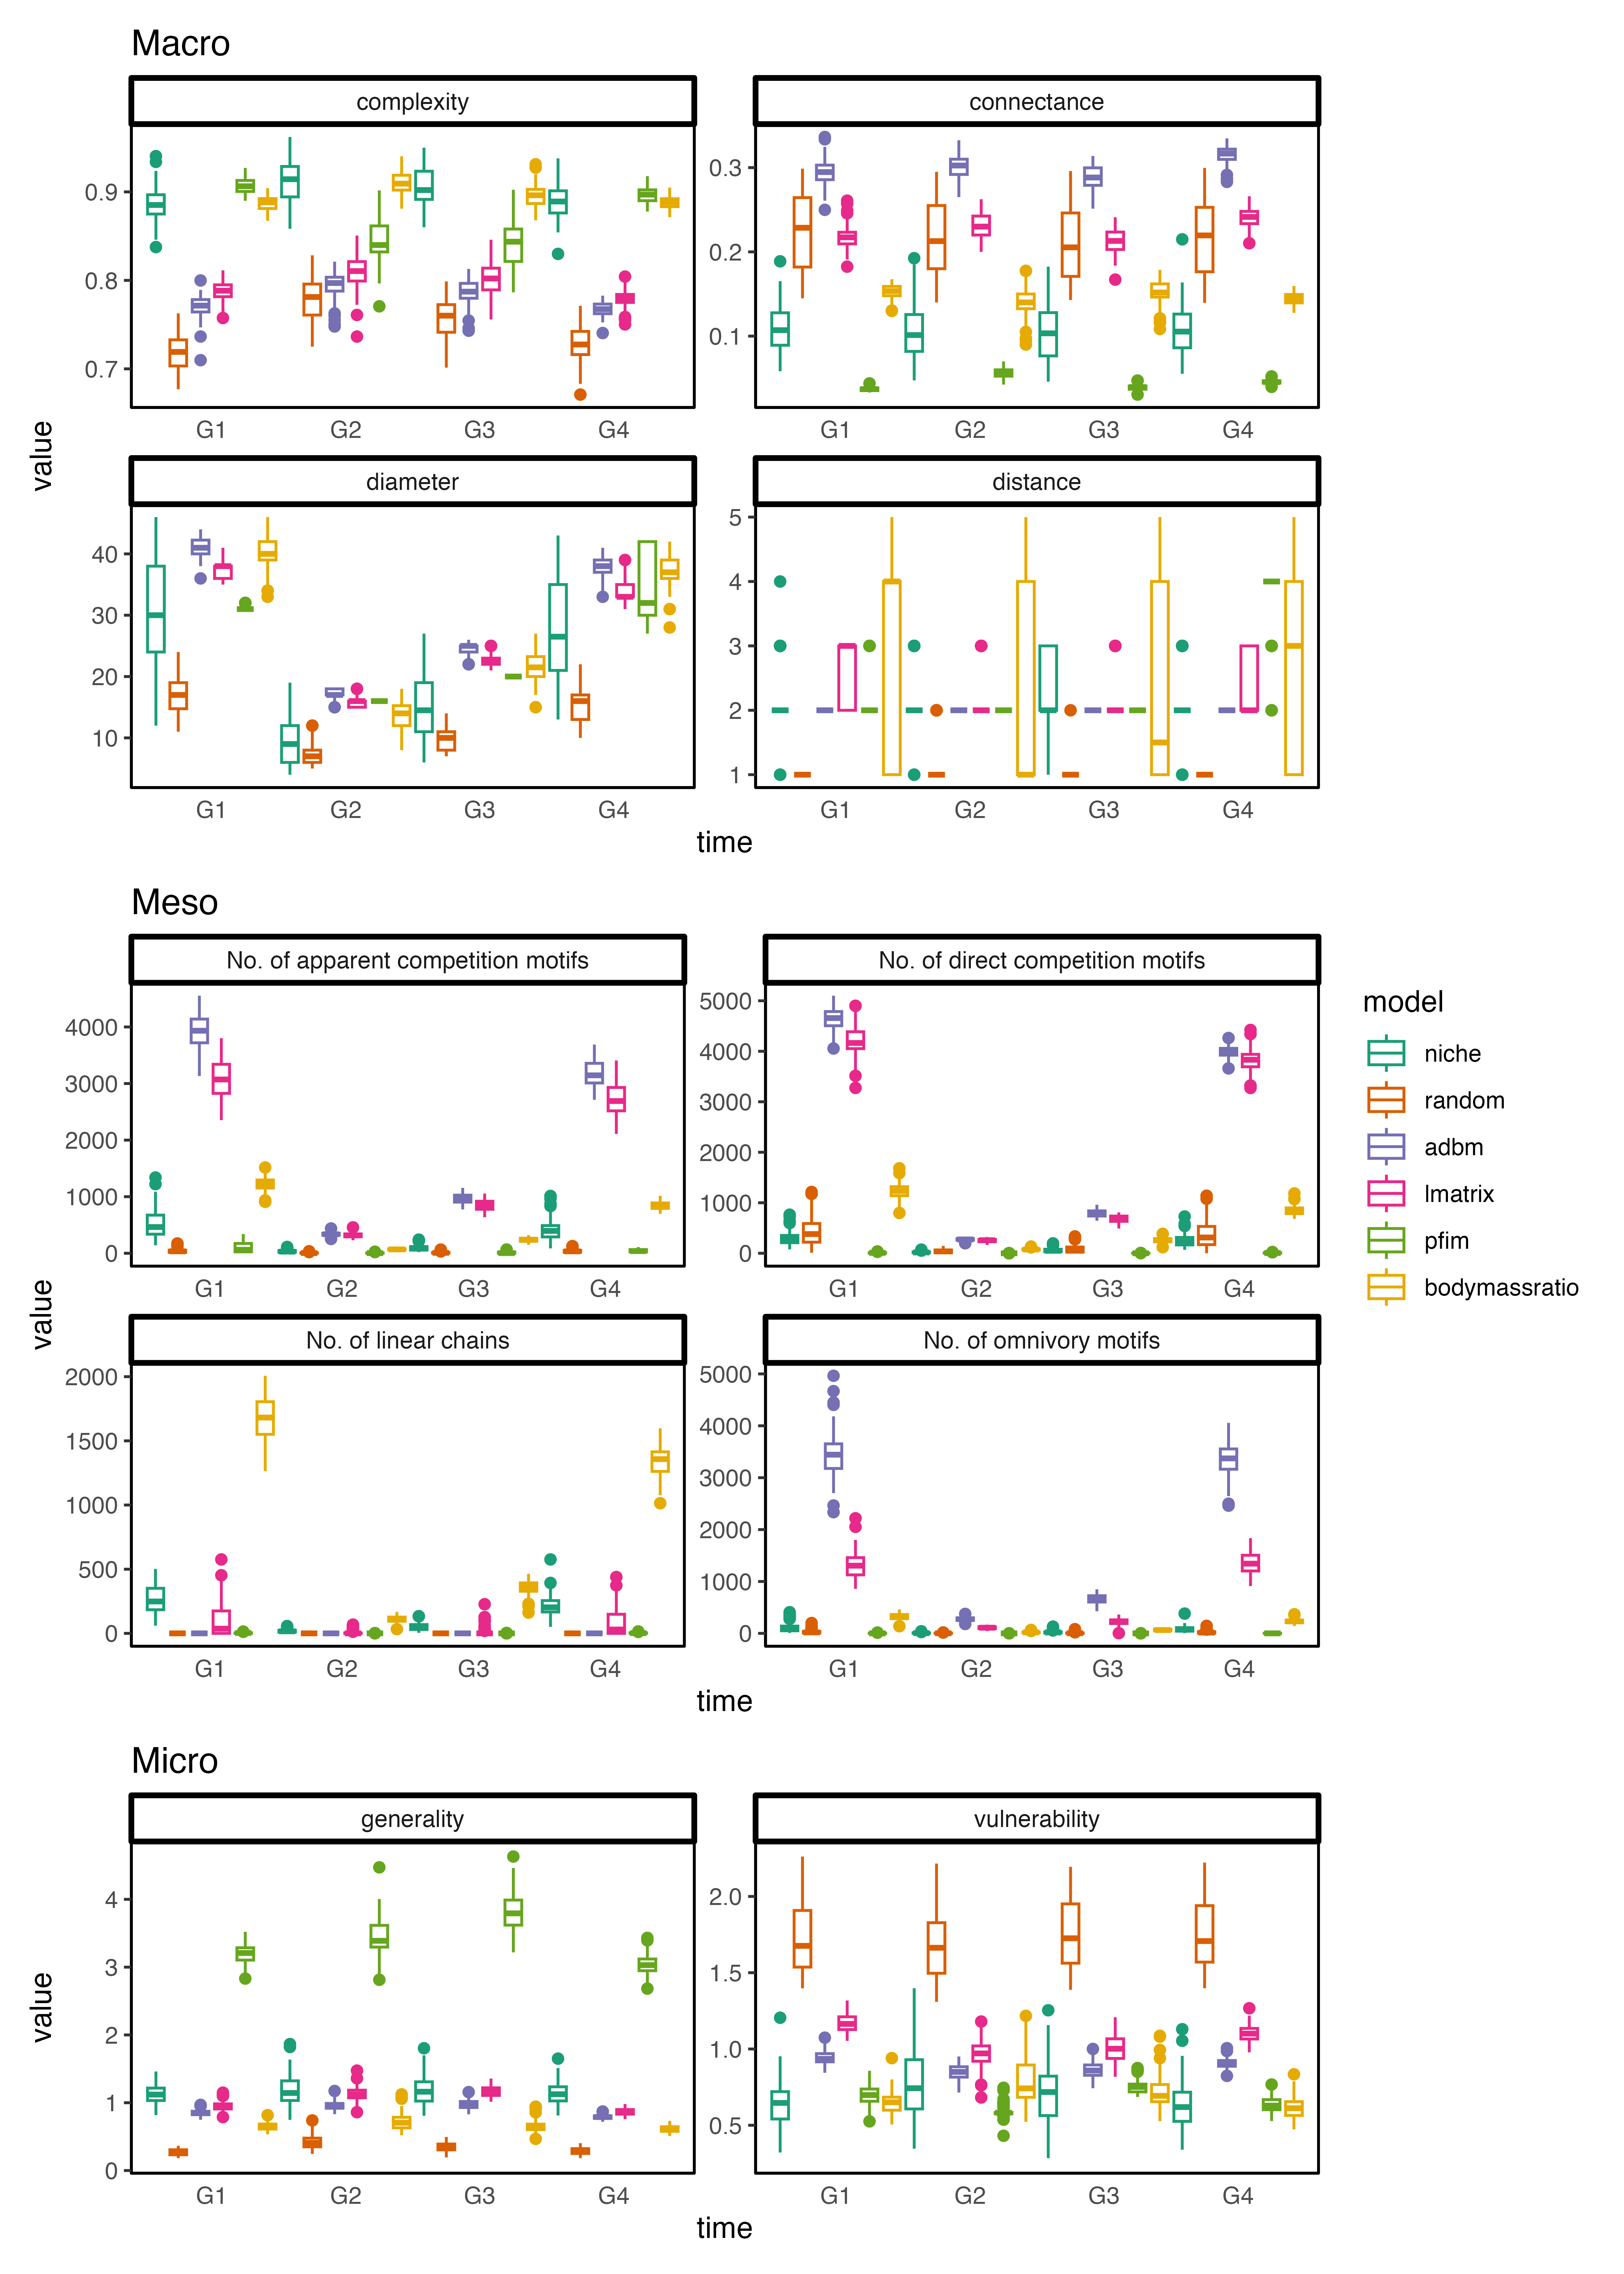
\includegraphics[keepaspectratio]{figures/summary.png}}

}

\caption{\label{fig-summary}stuff}

\end{figure}%

\subsection{Comparing inference}\label{comparing-inference}

\subsection{Extinctions}\label{extinctions}

\begin{figure}

\centering{

\pandocbounded{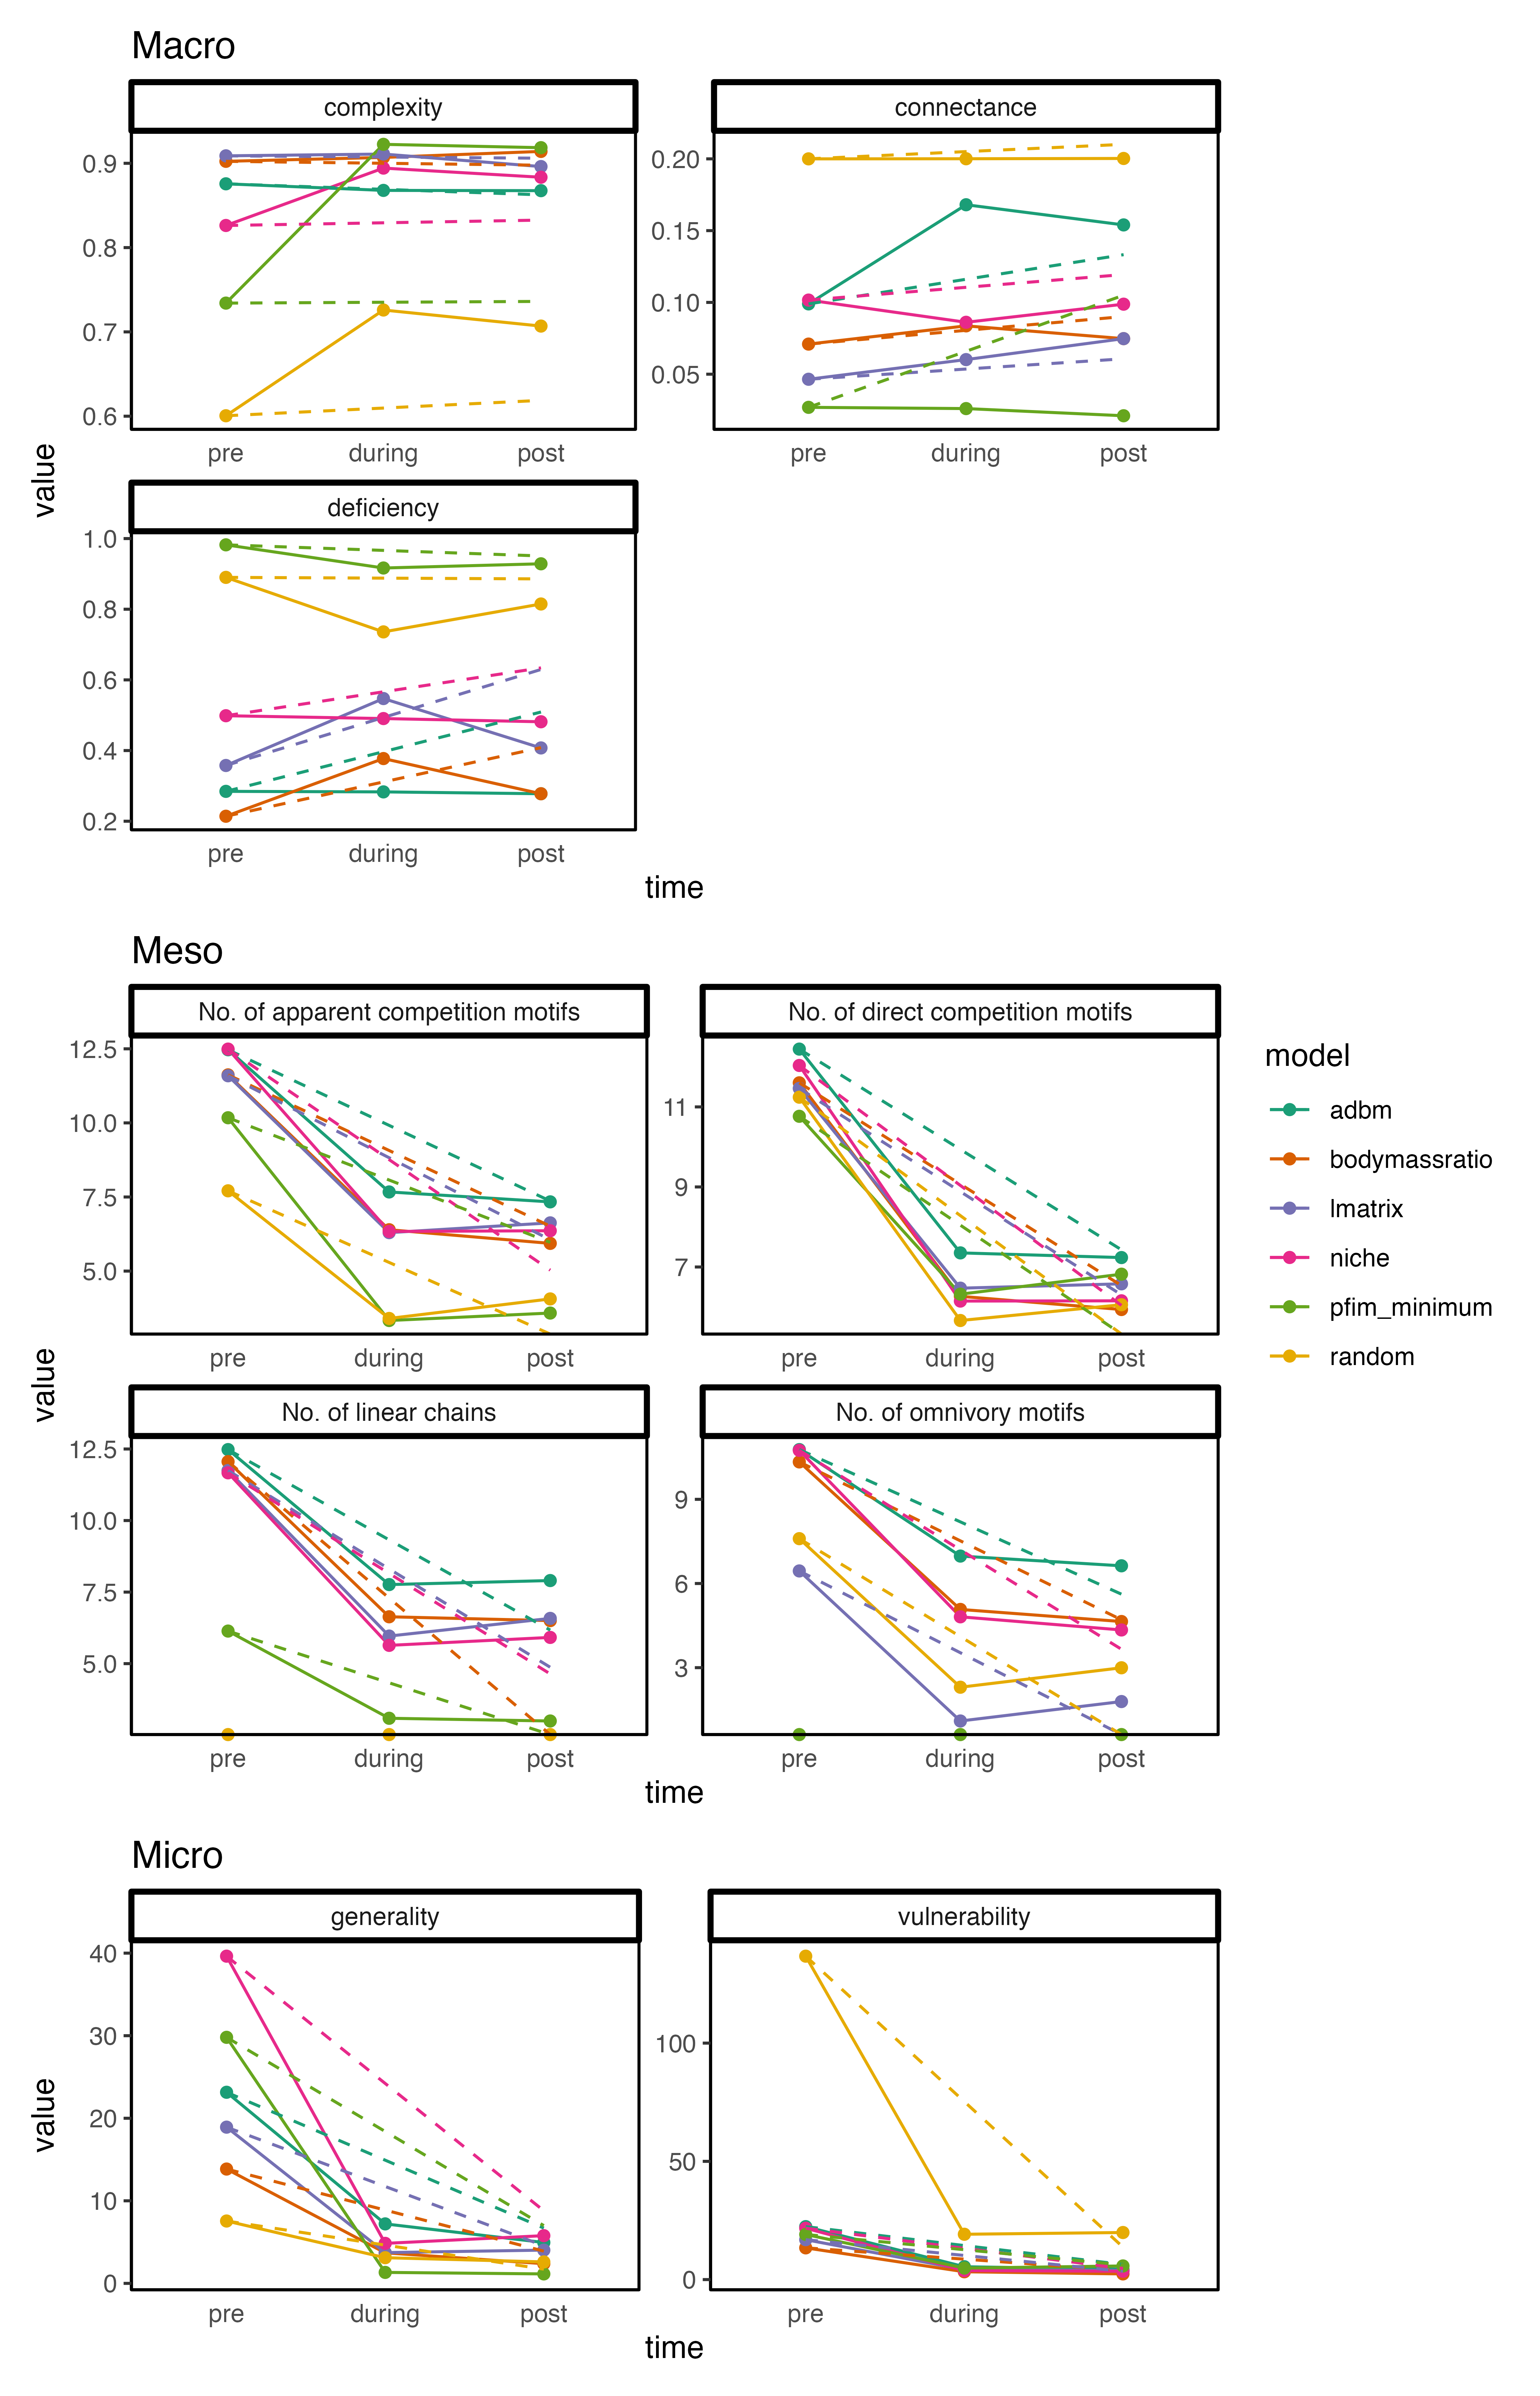
\includegraphics[keepaspectratio]{figures/extinction.png}}

}

\caption{\label{fig-extinction}Dashed line indicates the (mean)
extinction simulation results (post value, start values are those
estimated by the relevant model)}

\end{figure}%

\begin{figure}[H]

{\centering \pandocbounded{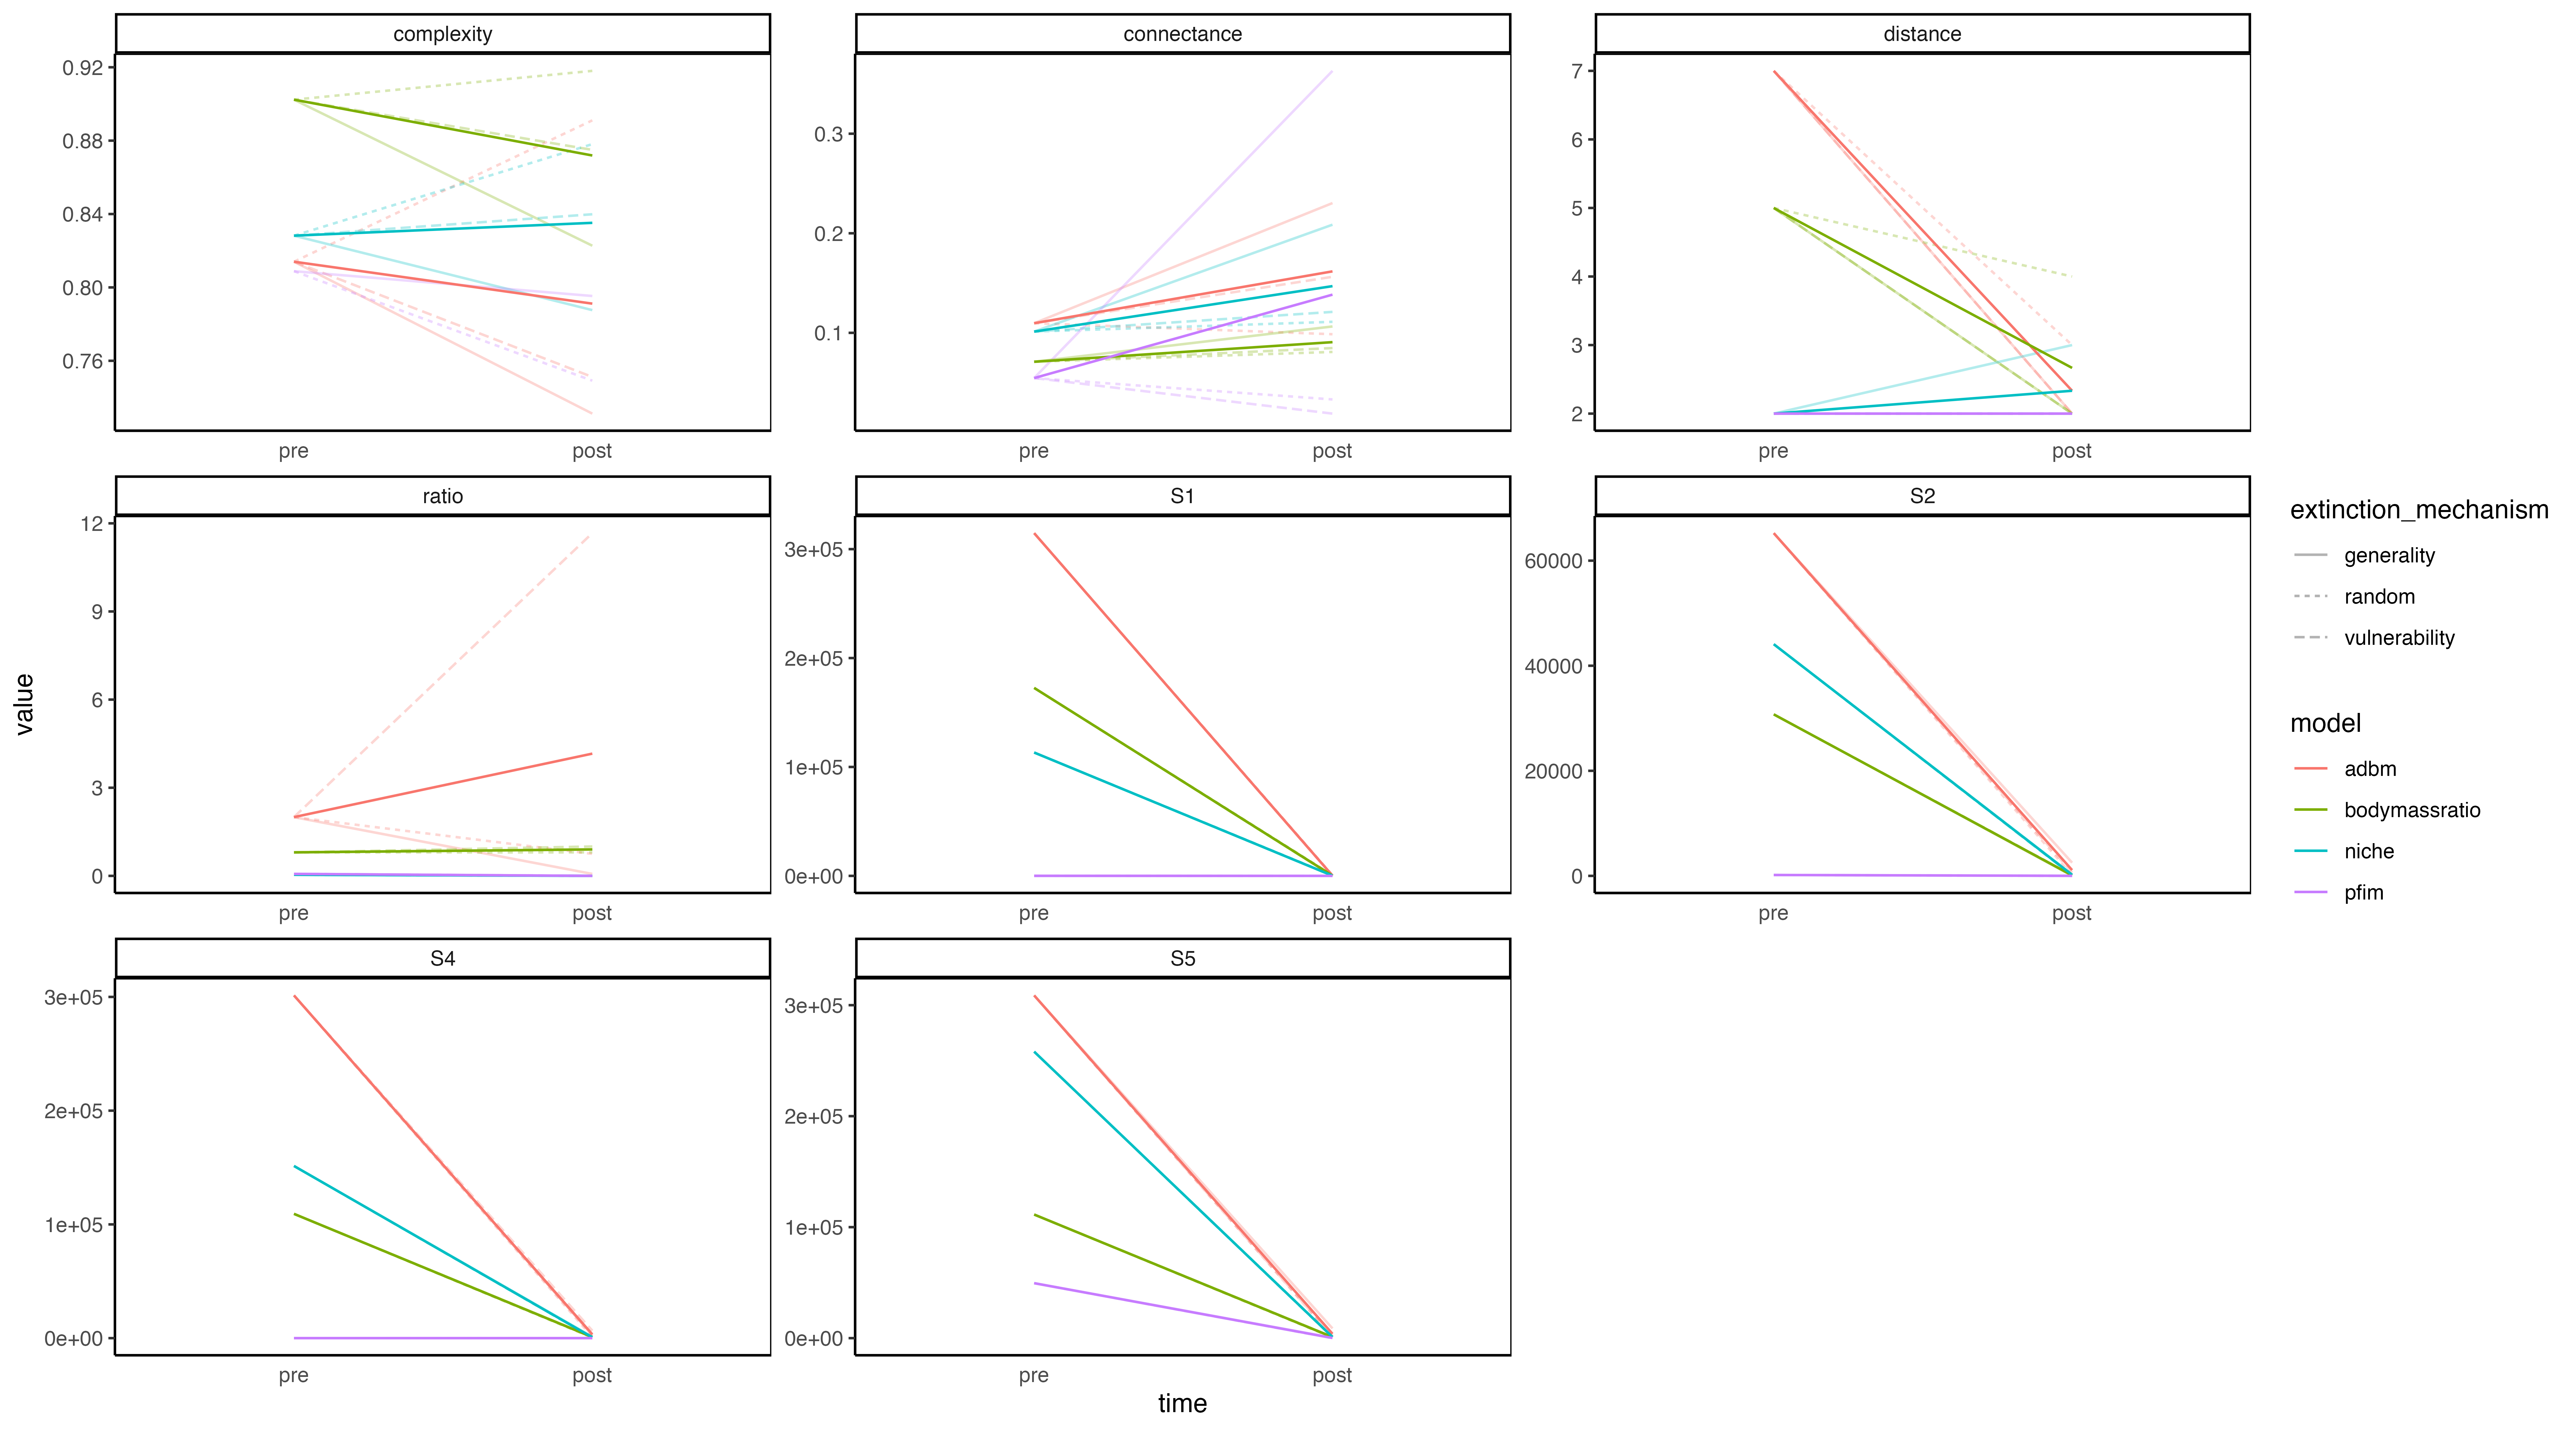
\includegraphics[keepaspectratio]{figures/extinction_all_results.png}}

}

\caption{Dark line indicates mean extinction simulation results the
lighter lines show each model individually, which is also denoted by
linetype}

\end{figure}%

\section*{References}\label{references}
\addcontentsline{toc}{section}{References}

\phantomsection\label{refs}
\begin{CSLReferences}{1}{0}
\bibitem[\citeproctext]{ref-caron2022}
Caron, D., Maiorano, L., Thuiller, W., \& Pollock, L. J. (2022).
Addressing the Eltonian shortfall with trait-based interaction models.
\emph{Ecology Letters}, \emph{25}(4), 889--899.
\url{https://doi.org/10.1111/ele.13966}

\bibitem[\citeproctext]{ref-dunhill2024}
Dunhill, A. M., Zarzyczny, K., Shaw, J. O., Atkinson, J. W., Little, C.
T. S., \& Beckerman, A. P. (2024). Extinction cascades, community
collapse, and recovery across a Mesozoic hyperthermal event.
\emph{Nature Communications}, \emph{15}(1), 8599.
\url{https://doi.org/10.1038/s41467-024-53000-2}

\bibitem[\citeproctext]{ref-fricke2022}
Fricke, E. C., Hsieh, C., Middleton, O., Gorczynski, D., Cappello, C.
D., Sanisidro, O., Rowan, J., Svenning, J.-C., \& Beaudrot, L. (2022).
Collapse of terrestrial mammal food webs since the Late Pleistocene.
\emph{Science}, \emph{377}(6609), 1008--1011.
\url{https://doi.org/10.1126/science.abn4012}

\bibitem[\citeproctext]{ref-petchey2008}
Petchey, O. L., Beckerman, A. P., Riede, J. O., \& Warren, P. H. (2008).
Size, foraging, and food web structure. \emph{Proceedings of the
National Academy of Sciences}, \emph{105}(11), 4191--4196.
\url{https://doi.org/10.1073/pnas.0710672105}

\bibitem[\citeproctext]{ref-rohr2010}
Rohr, R., Scherer, H., Kehrli, P., Mazza, C., \& Bersier, L.-F. (2010).
Modeling food webs: Exploring unexplained structure using latent traits.
\emph{The American Naturalist}, \emph{176}(2), 170--177.
\url{https://doi.org/10.1086/653667}

\bibitem[\citeproctext]{ref-roopnarine2006}
Roopnarine, P. D. (2006). Extinction cascades and catastrophe in ancient
food webs. \emph{Paleobiology}, \emph{32}(1), 1--19.
\url{https://www.jstor.org/stable/4096814}

\bibitem[\citeproctext]{ref-roopnarine2017}
Roopnarine, P. D. (2017). \emph{Ecological Modelling of Paleocommunity
Food Webs} (pp. 201--226). University of Chicago Press.

\bibitem[\citeproctext]{ref-shaw2024}
Shaw, J. O., Dunhill, A. M., Beckerman, A. P., Dunne, J. A., \& Hull, P.
M. (2024). \emph{A framework for reconstructing ancient food webs using
functional trait data} (p. 2024.01.30.578036). bioRxiv.
\url{https://doi.org/10.1101/2024.01.30.578036}

\bibitem[\citeproctext]{ref-strydom2023}
Strydom, T., Bouskila, S., Banville, F., Barros, C., Caron, D., Farrell,
M. J., Fortin, M.-J., Mercier, B., Pollock, L. J., Runghen, R., Dalla
Riva, G. V., \& Poisot, T. (2023). Graph embedding and transfer learning
can help predict potential species interaction networks despite data
limitations. \emph{Methods in Ecology and Evolution}, \emph{14}(12),
2917--2930. \url{https://doi.org/10.1111/2041-210X.14228}

\bibitem[\citeproctext]{ref-williams2000}
Williams, R. J., \& Martinez, N. D. (2000). Simple rules yield complex
food webs. \emph{Nature}, \emph{404}(6774), 180--183.
\url{https://doi.org/10.1038/35004572}

\bibitem[\citeproctext]{ref-williams2008}
Williams, R. J., \& Martinez, N. D. (2008). Success and its limits among
structural models of complex food webs. \emph{The Journal of Animal
Ecology}, \emph{77}(3), 512--519.
\url{https://doi.org/10.1111/j.1365-2656.2008.01362.x}

\bibitem[\citeproctext]{ref-yeakel2014}
Yeakel, J. D., Pires, M. M., Rudolf, L., Dominy, N. J., Koch, P. L.,
Guimarães, P. R., \& Gross, T. (2014). Collapse of an ecological network
in ancient egypt. \emph{PNAS}, \emph{111}(40), 14472--14477.
\url{https://doi.org/10.1073/pnas.1408471111}

\end{CSLReferences}





\end{document}
